

\documentclass[journal]{IEEEtran}
\IEEEoverridecommandlockouts

\usepackage{amsmath,amssymb,amsfonts}
\usepackage{graphicx}
\usepackage{booktabs}
\usepackage{url}
\usepackage{xcolor}
\usepackage{tikz}
\usetikzlibrary{arrows.meta,positioning}

\DeclareMathOperator{\rank}{rank}
\DeclareMathOperator{\range}{range}

\newcommand{\bG}{\mathbf{G}}
\newcommand{\bS}{\mathbf{S}}
\newcommand{\bB}{\mathbf{B}}
\newcommand{\bW}{\mathbf{W}}
\newcommand{\bZ}{\mathbf{Z}}
\newcommand{\bY}{\mathbf{Y}}
\newcommand{\bJ}{\mathbf{J}}
\newcommand{\bD}{\mathbf{D}}
\newcommand{\bU}{\mathbf{U}}
\newcommand{\bg}{\mathbf{g}}
\newcommand{\CN}{\mathcal{CN}}
\newcommand{\Hank}{\mathcal{H}}
\newcommand{\reff}{r_{\mathrm{eff}}}
\newcommand{\rmax}{r_{\max}}
\newcommand{\dhs}{\Delta_{\mathrm{HS}}}

\begin{document}

\title{Hankel-Structured Channel Estimation for Magnitude-Only Rydberg Atomic Receivers: When Does Structure Help?}

\author{Abdullah~Haatim%
\thanks{A.~Haatim is with the Department of Electrical and Electronics
Engineering, Birla Institute of Technology and Science, Pilani~--- Pilani
Campus, India (e-mail: f20220519@pilani.bits-pilani.ac.in).}}

\maketitle

\begin{abstract}
We investigate when spatial structure improves magnitude-only channel
estimation for Rydberg atomic receivers with a known reference field. A
Hankel-structured extension of expectation--maximization
Gerchberg--Saxton (EM-GS) selects one structural rank from held-out pilots
and refits the channel using all pilots. In 2,400 paired trials at the
principal operating point, HS-GS gives a 2.70~dB mean improvement over six
per-SNR paired medians. The benefit increases with array capacity and
decreases with multipath complexity; at high complexity, forced rank
reduction can be harmful. Normalized effective rank organizes these trends,
but does not define a universal performance threshold, and normalized path
count is a stronger predictor on the tested matched geometric-channel
configurations. Positive gains also persist under two alternative multipath
distributions. A controlled comparison with matching Cadzow sweeps finds a
modest accuracy advantage for interleaving the structural step, while rank
selection dominates computation for larger arrays. These conclusions are
limited to the specified simulated ULA magnitude-observation model.
\end{abstract}

\begin{IEEEkeywords}
Rydberg atomic receiver, channel estimation, phase retrieval, Hankel matrix,
constrained Cram\'er--Rao bound, effective rank.
\end{IEEEkeywords}


\section{Introduction}

\IEEEPARstart{S}{ixth-generation} wireless systems are expected to operate
over wider bandwidths and at increasingly high carrier frequencies, placing
new demands on receiver sensitivity and reconfigurability. Quantum sensing has
emerged as one possible response, and Rydberg atomic receivers have recently
attracted attention for wireless communications~\cite{cui2025,gong2025mag}.
These receivers use laser-excited atoms to sense an incident radio-frequency
field through changes in optical transmission. Unlike a conventional coherent
receiver, however, the optical readout directly provides the field amplitude
rather than its complex value, so the channel phase is not directly observed.

Recovering a complex channel from these amplitude-only measurements is a
phase-retrieval problem. A known reference field makes this recovery possible
by converting relative phase into observable amplitude. Existing approaches
include iterative phase-retrieval methods~\cite{gerchberg1972}, gradient
descent with structural projection~\cite{xu2025}, and unrolled
networks~\cite{xiao2026}. These works mainly focus on improving channel
estimation performance. Less attention has been given to a more basic
question: when does imposing channel structure actually help, and when does
that structure become too restrictive? This paper addresses that question
using the spatial structure of multipath channels on a uniform linear array.

We propose a Hankel-structured extension of EM-GS for magnitude-only channel
estimation. The estimator exploits the exponential structure of the channel
across the array, selects the structural order using held-out pilot
measurements, and falls back exactly to EM-GS when the measurements do not
support a useful constraint. We then study how the benefit of the Hankel
constraint changes with the array size and the complexity of the channel.
Path count alone does not fully describe this behaviour, so we also describe
channel complexity using its effective rank relative to the available Hankel
rank. We compare that descriptor with normalized path count, test two
additional channel distributions, and isolate the effect of where the
structural projection is placed in the iterative solver.



\section{System Model}
\label{sec:model}

\begin{figure*}[!t]
\centering
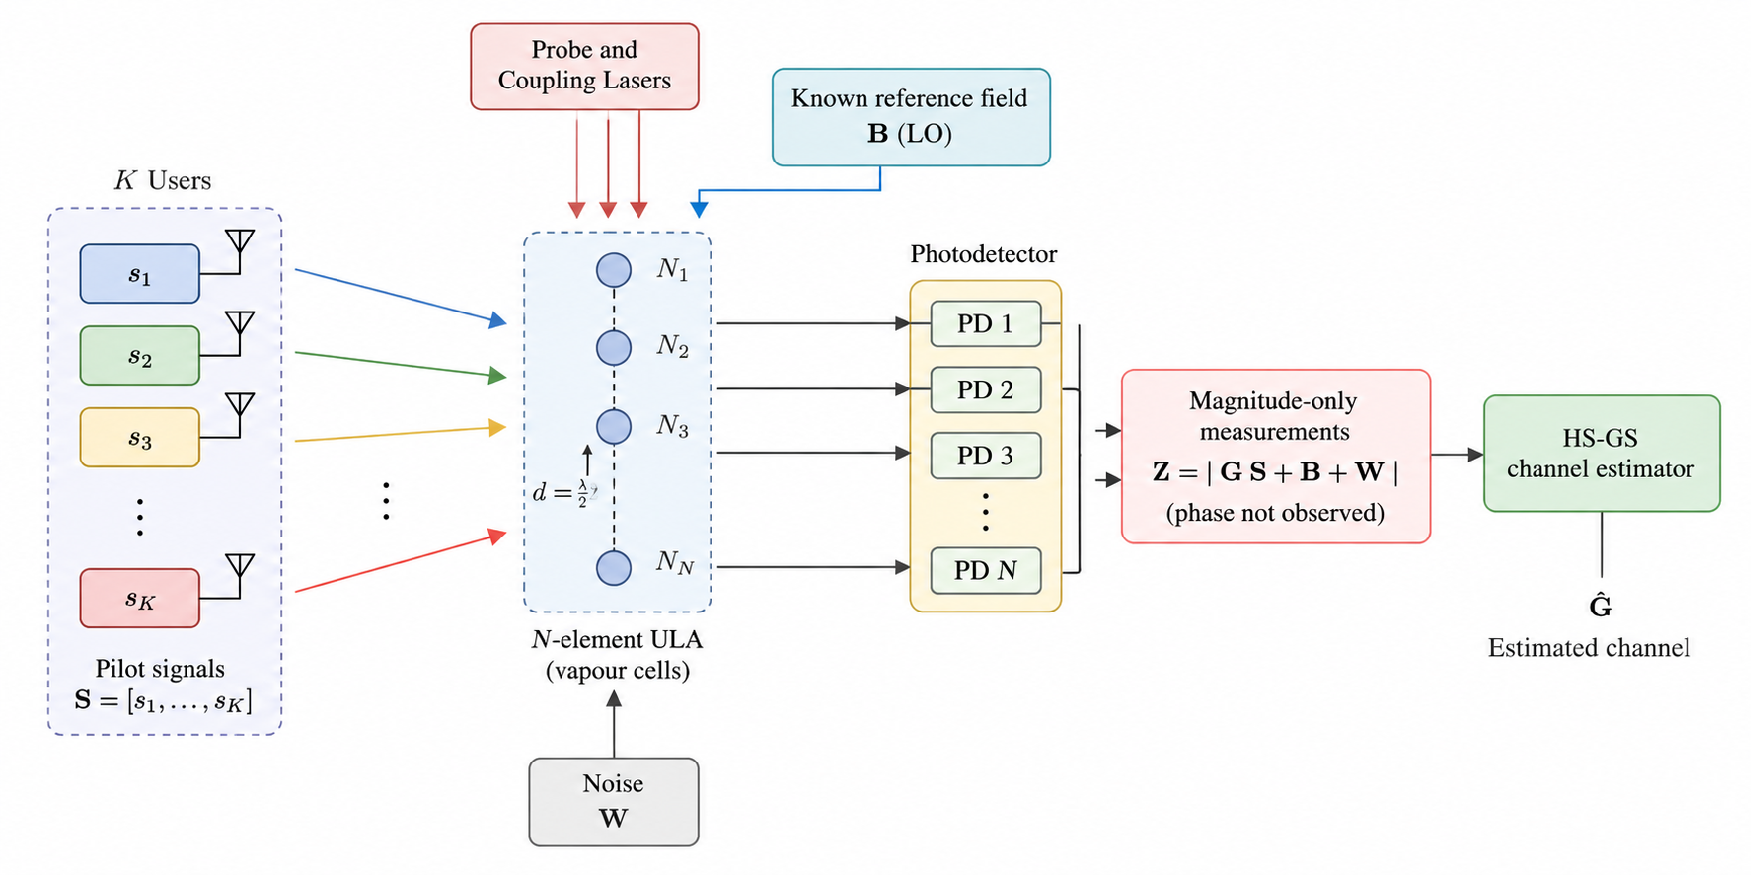
\includegraphics[width=0.90\textwidth]{fig/ULA.pdf}
\caption{Uplink of the Rydberg atomic receiver. $K$ single-antenna users
transmit known pilot signals to $N$ vapour-cell receive elements arranged as
a uniform linear array. The user RF signals and a known reference RF field
interact with the Rydberg atoms. Probe and coupling lasers are used for the
atomic readout, and the photodetector measures the magnitude of the total
field. The estimator therefore observes $\bZ$ without directly observing
its phase.}
\label{fig:system}
\end{figure*}

We consider an uplink system with $K$ single-antenna users and one Rydberg atomic receiver, as shown in Fig.~\ref{fig:system}. The receiver contains $N$ vapor-cell receive elements arranged in a uniform linear array (ULA). Each vapor cell contains atoms that are excited to Rydberg states using
probe and coupling lasers. The RF signals transmitted by the users interact
with these atoms. A known RF reference field is also applied at the
receiver. The atomic response changes the probe laser passing through the
vapour cell, and this change is measured using a photodetector. The receiver
therefore measures the strength of the total RF field, but it does not
directly observe its complex phase~\cite{cui2025}.

We model the channel between each user and the array using several
propagation paths. A path may represent a signal arriving directly from the
user or after interacting with objects in the environment. For user $k$,
the channel coefficient at the $n$th receive element is

\begin{equation}
g_k[n]
=
\sum_{\ell=1}^{L_k}
\alpha_{\ell,k}
e^{-\jmath(n-1)\psi_{\ell,k}},
\qquad
\psi_{\ell,k}
=
\pi\sin\theta_{\ell,k},
\label{eq:chan}
\end{equation}

where $L_k$ is the number of propagation paths for user $k$,
$\alpha_{\ell,k}$ is the complex gain of path $\ell$, and
$\theta_{\ell,k}$ is its angle of arrival. In our simulations,
$L_k$ is selected between $3$ and $7$, following the channel setting
in~\cite{xu2025}.

The exponential term in \eqref{eq:chan} describes how the phase of one
propagation path changes as we move from one array element to the next.
To see this, consider a single path arriving at the array from an angle
$\theta$. The signal reaches the different array elements at slightly
different times because the elements are at different positions. This
difference in travel distance produces a phase difference between adjacent
elements.

With half-wavelength spacing between the array elements, the phase change
between two neighbouring elements is

\begin{equation}
\psi
=
\pi\sin\theta.
\end{equation}

The first array element has no additional phase shift from the array
position. The second element has a phase shift of $\psi$, the third has a
phase shift of $2\psi$, and so on. Therefore, the samples produced by one
path across the array have the form

\begin{equation}
1,\quad
e^{-\jmath\psi},\quad
e^{-\jmath2\psi},\quad
\ldots,\quad
e^{-\jmath(N-1)\psi}.
\end{equation}

The factor

\begin{equation}
e^{-\jmath(n-1)\psi_{\ell,k}}
\end{equation}

in \eqref{eq:chan} represents exactly this phase pattern for path $\ell$.
The coefficient $\alpha_{\ell,k}$ determines the strength and initial
phase of that path. Since several paths can arrive at the receiver, their
contributions are added together to produce the final channel coefficient
$g_k[n]$.

The channel coefficients of user $k$ are collected into the vector

\begin{equation}
\bg_k
=
\begin{bmatrix}
g_k[1] &
g_k[2] &
\cdots &
g_k[N]
\end{bmatrix}^{T},
\end{equation}

and the channels of all $K$ users are collected into

\begin{equation}
\bG
=
\begin{bmatrix}
\bg_1 &
\bg_2 &
\cdots &
\bg_K
\end{bmatrix}
\in\mathbb{C}^{N\times K}.
\end{equation}

During channel estimation, the $K$ users transmit $P$ known pilot symbols.
These pilots are collected in

\begin{equation}
\bS
\in
\mathbb{C}^{K\times P}.
\end{equation}

Each row of $\bS$ contains the pilots transmitted by one user, while each
column represents one pilot transmission. The same pilot matrix is used
when comparing the different channel estimators.

If the receiver could observe the complete complex signal, the contribution
from the users would be $\bG\bS$. However, the Rydberg receiver considered
here measures magnitude rather than directly measuring this complex value.
A known reference RF field is therefore applied at the receiver. We denote
this reference by

\begin{equation}
\bB
\in
\mathbb{C}^{N\times P}.
\end{equation}

The reference field is known in both amplitude and phase. It is important
because the magnitude of an unknown signal alone does not directly reveal
its phase. When the unknown user signal is combined with a known reference,
the resulting magnitude depends on their relative phase. This provides
information that can be used to estimate the complex channel.

Including noise, the field before the magnitude measurement is

\begin{equation}
\bY
=
\bG\bS+\bB+\bW,
\end{equation}

where the noise is modeled as complex Gaussian,

\begin{equation}
\bW_{np}
\sim
\CN(0,\sigma^2).
\end{equation}

The noise is therefore added before the magnitude is measured. The Rydberg
receiver observes

\begin{equation}
\bZ
=
\left|
\bG\bS+\bB+\bW
\right|,
\label{eq:obs}
\end{equation}

where $|\cdot|$ is applied to every element of the matrix.

Equation~\eqref{eq:obs} is the main measurement model used in this work.
The pilots $\bS$ and reference field $\bB$ are known, and the receiver
measures $\bZ$. The unknown quantity is the complex channel matrix $\bG$.
The channel-estimation problem is therefore to recover $\bG$ even though
the receiver does not directly observe the phase of the received signal.

We assume a narrowband, frequency-flat channel during the pilot interval.
The path gains are modeled as independent circularly symmetric complex
Gaussian variables, and the angles of arrival are independently generated
over $(-90^\circ,90^\circ)$. The users have equal received power, and the
reference field remains known at the receiver. For a fair comparison, all
estimators use the same channel, pilots, reference field, and noise
realization within each Monte Carlo trial.

The reference-to-signal ratio (RSR) is the reference power divided by the
single-user received signal power. We define SNR using aggregate received
signal power,
\begin{equation}
\mathrm{SNR}=\frac{\mathbb{E}\|\bG\bS\|_F^2/(NP)}{\sigma^2}.
\end{equation}
For the equal-power normalization used in the simulations this reduces to
$K/\sigma^2$. All SNR axes in Section~\ref{sec:results} use this aggregate
convention.


\section{Proposed Estimator}
\label{sec:method}

\subsection{Structure and its Capacity}

The rank of a matrix tells us how many independent components are needed
to describe it. A low-rank matrix is therefore described using only a
small number of important components. To use this idea for our channel,
we first arrange the channel into a Hankel matrix. A Hankel matrix is a
matrix in which the same channel samples are repeated along the
antidiagonals. For example, consider

\begin{equation}
\bg=
\begin{bmatrix}
g_1 & g_2 & g_3 & g_4 & g_5
\end{bmatrix}^{T}.
\end{equation}

One possible Hankel representation is

\begin{equation}
\Hank(\bg)
=
\begin{bmatrix}
g_1 & g_2 & g_3\\
g_2 & g_3 & g_4\\
g_3 & g_4 & g_5
\end{bmatrix}.
\end{equation}

We use this representation because the channel in \eqref{eq:chan} is not
a random collection of values. It is made up of propagation paths, and
each path produces a complex exponential pattern across the array elements.
When this type of channel is written as a Hankel matrix, each path
contributes one rank-one component. For example, a channel containing one
path produces a Hankel matrix with rank at most one. Two paths produce a
matrix with rank at most two. In general, for a channel with $L_k$ paths,

\begin{equation}
\rank\Hank_p(\bg_k)
\leq
L_k.
\end{equation}

Therefore, when the channel has only a few important paths, its Hankel
matrix can have a low rank~\cite{cadzow1988,markovsky2008}. This is why we
use the Hankel representation: it changes the multipath structure of the
channel into a low-rank matrix structure that can be used during channel
estimation.

The maximum possible rank of the Hankel matrix depends on the number of
array elements. For an $(N-p)\times(p+1)$ Hankel matrix, the maximum rank is

\begin{equation}
\min(N-p,p+1).
\end{equation}

Choosing $p$ so that the matrix is as balanced as possible gives

\begin{equation}
\rmax(N)
=
\left\lceil
\frac{N}{2}
\right\rceil.
\label{eq:cap}
\end{equation}

For example, if $N=16$, the maximum Hankel rank is $8$. If the channel
has only three important paths, its Hankel rank can be at most $3$.
This is much smaller than the maximum rank of $8$, so there is useful
low-rank structure that can be used during estimation. If the channel
rank is already close to $8$, there is less low-rank structure available.
In this case, forcing the channel to have a much smaller rank may remove
part of the real channel.

\subsection{The Estimator}

Starting from the spectral initialization used by EM-GS, iteration $t$ forms
\begin{align}
\boldsymbol\Lambda^{(t)}&=\bG^{(t)}\bS+\bB,\\
\boldsymbol{\kappa}^{(t)}&=2\bZ\odot|\boldsymbol\Lambda^{(t)}|/\sigma^2,\\
\bY^{(t)}&=\bZ\odot R(\boldsymbol{\kappa}^{(t)})
 \odot\exp\!\left(\jmath\arg\boldsymbol\Lambda^{(t)}\right),\\
\widetilde{\bG}^{(t+1)}&=(\bY^{(t)}-\bB)\bS^H
 (\bS\bS^H)^{-1},
\end{align}
where $R(x)=I_1(x)/I_0(x)$ is applied elementwise and $\odot$ denotes
elementwise multiplication. HS-GS uses exactly this measurement update and
then applies a Cadzow structural step to every user column. Thus, disabling
the structural step gives the EM-GS implementation exactly.

For one column, a Cadzow sweep first converts the estimate into the Hankel
matrix described earlier.

Next, singular value decomposition (SVD) is applied to the Hankel matrix.
SVD separates the matrix into components and gives a singular value for
each component. A larger singular value means that the component has a
larger contribution to the matrix. For example, suppose the singular
values are

\begin{equation}
\sigma_1=10,
\qquad
\sigma_2=6,
\qquad
\sigma_3=0.3.
\end{equation}

Here, the three singular values are $10$, $6$, and $0.3$. If we decide to
use a rank of $2$, we keep the two largest components, corresponding to
$10$ and $6$, and remove the smaller component corresponding to $0.3$.
The resulting matrix therefore has rank $2$. If the true channel has only
two important components, the removed component may mainly come from noise
or estimation error.

After the rank reduction, the matrix is converted back into a channel
vector. The entries along each antidiagonal are averaged because they
represent the same channel sample. One sweep can be written as

\begin{equation}
\mathcal{P}_r(\bg)
=
\Hank_p^{\dagger}
\left(
\Pi_r(\Hank_p(\bg))
\right),
\end{equation}

where $\Pi_r$ keeps the $r$ largest singular values and
$\Hank_p^{\dagger}$ converts the Hankel matrix back into a channel vector
by averaging its antidiagonals.

The reported estimator applies four such sweeps after every EM-GS update.
Finite alternating sweeps are a low-rank structural heuristic: after the
Hankel averaging step, relifting need not have rank exactly $r$, and the
operation does not impose every physical unit-circle constraint in
\eqref{eq:chan}. Choosing $r$ remains important because a large rank changes
little, whereas an overly small rank can remove genuine channel components.

\subsection{Choosing the Hankel Rank}

The true path count is not used. We reserve the final
$\max(1,\operatorname{round}(0.3P))$ pilot columns for validation and fit
each candidate $r\in\{1,\ldots,r_{\max}\}$ using the remaining columns.
The selected rank minimizes the held-out squared magnitude residual
\begin{equation}
\hat r=\arg\min_r
\left\|\bZ_{\rm val}-
 \left|\widehat{\bG}_r\bS_{\rm val}+\bB_{\rm val}\right|\right\|_F^2.
\end{equation}
One scalar rank is shared by all user columns. After selection, the final
estimator is restarted and fitted using \emph{all} $P$ pilots, so the
validation pilots are not permanently discarded. If $\hat r=r_{\max}$,
the structural step is bypassed and the final estimate equals the paired
EM-GS estimate exactly. This fallback does not guarantee that every active
rank choice improves the unknown true-channel error.


\section{Performance References}
\label{sec:crlb}

\subsection{Information in an Amplitude Measurement}

The Cramér--Rao lower bound (CRLB) is used as a theoretical reference for
channel estimation. In simple terms, it tells us how accurately an
unbiased estimator could estimate the channel from the available
measurements. The amount of information contained in the measurements
therefore affects the CRLB.

This is important for the Rydberg receiver because it measures only the
amplitude of the received signal, not its full complex value. For example,
suppose the noiseless received signal is

\begin{equation}
s=3+j4.
\end{equation}

A complex receiver can observe both the real part, $3$, and
the imaginary part, $4$. The amplitude-only receiver instead observes

\begin{equation}
|s|
=
\sqrt{3^2+4^2}
=
5.
\end{equation}

Knowing only the value $5$ does not tell us that the original signal was
$3+j4$. Other complex values can have the same amplitude. Therefore, an
amplitude measurement contains less information than a full complex
measurement.

When complex Gaussian noise is added before the amplitude is measured, the
measured amplitude follows a Rician distribution. We use this Rician model
to calculate the Fisher information matrix $J$ and the corresponding
CRLB~\cite{balan2015,cui2025}. The Fisher information matrix describes how
much information the measurements contain about the unknown channel.

A simple example can be used to understand $J$. Let the complex signal be

\begin{equation}
s=x+jy,
\end{equation}

where $x$ is the real part and $y$ is the imaginary part. The receiver
measures only

\begin{equation}
a=|s|
=
\sqrt{x^2+y^2}.
\end{equation}

For example, if $x=3$ and $y=4$, then $a=5$. We can then check how much
the measured amplitude changes when $x$ or $y$ changes:

\begin{equation}
\begin{bmatrix}
\frac{\partial a}{\partial x}\\[2mm]
\frac{\partial a}{\partial y}
\end{bmatrix}
=
\begin{bmatrix}
3/5\\
4/5
\end{bmatrix}.
\end{equation}

This tells us the direction in which this amplitude measurement provides
information about the unknown complex signal. The Fisher information from
this measurement has the form

\begin{equation}
J
\propto
\begin{bmatrix}
3/5\\
4/5
\end{bmatrix}
\begin{bmatrix}
3/5 & 4/5
\end{bmatrix}
=
\begin{bmatrix}
9/25 & 12/25\\
12/25 & 16/25
\end{bmatrix}.
\end{equation}

This matrix has rank one. This means that one amplitude measurement gives
information in only one direction. We do not have enough information from
this one measurement to find the real and imaginary parts separately. This
agrees with the earlier example: knowing that the amplitude is $5$ is not
enough to know that the signal is exactly $3+j4$.

In practice, we use several pilot measurements. Each pilot gives some
information about the unknown channel. The information from all of these
measurements is combined to form the full Fisher information matrix $J$.
Therefore, $J$ describes the information provided by all the measurements
used for channel estimation.

The Hankel structure also allows us to use the larger array differently.
The channel coefficients across the array are not completely independent
because they are produced by the same propagation paths. The Hankel
constraint uses this relationship between the array elements. This allows
HS-GS to make use of the additional spatial structure provided by a larger
array.

\subsection{Constrained Cramér--Rao Bound}

The CRLB described above treats each channel coefficient as a separate
unknown. However, our channel coefficients are connected because they are
produced by the same propagation paths. For example, consider

\begin{equation}
\bg=
\begin{bmatrix}
g_1 & g_2 & g_3 & g_4
\end{bmatrix}^{T}.
\end{equation}

The ordinary CRLB allows $g_1$, $g_2$, $g_3$, and $g_4$ to take any
values. In our channel model, things are not completely independent. These
values are connected through the path gains and angles in
\eqref{eq:chan}. The constrained CRLB (CCRB) includes this additional
information.

The CCRB is calculated as~\cite{gorman1990,stoica1998}

\begin{equation}
\mathrm{CCRB}
=
\bU(\bU^T J\bU)^{-1}\bU^T,
\end{equation}

where $J$ is the Fisher information matrix calculated in the previous
section. The matrix $U$ describes the ways in which the channel is allowed
to change while still following the multipath channel model.

We use both the CRLB and CCRB only as reference curves. The ordinary CRLB
treats the channel coefficients separately, while the CCRB also uses the
known multipath structure. The difference between them therefore gives us
an idea of how much improvement may be possible by using this structure.

These bounds are derived for unbiased estimators, while EM-GS and HS-GS
are not assumed to be unbiased. Therefore, we do not treat the CRLB or
CCRB as absolute lower limits on their measured NMSE.


\section{Numerical Results}
\label{sec:results}

\subsection{Experimental Setup}

The verification campaign contains 27,300 fresh paired Monte Carlo trials
across 73 operating cells, with 300 or 400 trials per cell, plus 2,400
bound evaluations on the main-figure channel realizations. Trial counts were
fixed before simulation. Within a trial, all estimators use the same channel,
pilots, reference field, and noise.

The principal comparison uses $N=32$, $K=3$, $P=30$, RSR $=12$~dB,
100 final EM-GS updates, 25 updates per candidate rank, and four Cadzow
sweeps per structural application. The path-count sweep uses 50 final and
20 candidate updates. The matched effective-rank experiments use $P=20$,
RSR $=10$~dB, 100/25 updates, and SNR drawn uniformly from
$[-10,20]$~dB on a millidecibel grid.

We report two different summaries. For trial $i$, let
$e_{m,i}=\|\widehat{\bG}_{m,i}-\bG_i\|_F^2$ and
$d_i=\|\bG_i\|_F^2$. The plotted NMSE and the paired-median gain are
\begin{align}
\mathrm{NMSE}_{m,\mathrm{dB}}
 &=10\log_{10}\frac{\sum_i e_{m,i}}{\sum_i d_i},\\
\Delta_{\mathrm{med}}
 &=\operatorname{median}_i\!
 \left[10\log_{10}\frac{e_{\mathrm{EM},i}}{e_{\mathrm{HS},i}}\right].
\end{align}
The vertical separation of two NMSE curves is a ratio-of-sums gain; it need
not equal $\Delta_{\mathrm{med}}$. Pointwise 95\% intervals use 4,000 paired
bootstrap resamples. Pooled random-SNR medians are conditional on the stated
SNR distribution.

\subsection{Principal Performance and Array Size}
\label{sec:main}

Fig.~\ref{fig:main}(a) compares the estimators and reference curves. Across
the six SNR values, paired-median gains range from 2.54 to 2.97~dB and
their mean is 2.70~dB. The corresponding vertical NMSE-curve gaps range
from 2.38 to 2.90~dB. Projection is active in all 2,400 principal trials.

The Rician CRLB and geometric CCRB are evaluated using the same channel
realizations and energy normalizations. At SNRs of 5~dB and above, EM-GS
differs from the Rician CRLB by at most 0.107~dB. The geometric CCRB is
6.95--7.06~dB below the unconstrained bound, and HS-GS remains
4.37--4.85~dB above it. The CCRB is an ideal local reference conditional on
the true path configuration; neither curve is an unconditional lower limit
for the biased estimators tested here.

Fig.~\ref{fig:main}(b) and Table~\ref{tab:array} show that the structural
gain grows with array capacity. Each table row averages summaries from two
pilot counts and six SNR values, with 400 trials per operating point.
The averaged EM-GS baseline spans only 0.120~dB, whereas the paired-median
HS-GS gain grows from 0.236 to 3.264~dB. At $N=8$, projection is inactive
in 42.94\% of trials. The slightly positive paired median and negative
ratio-of-sums gain at $N=8$ show why the aggregation rule must be stated.

\begin{figure*}[!t]
\centering
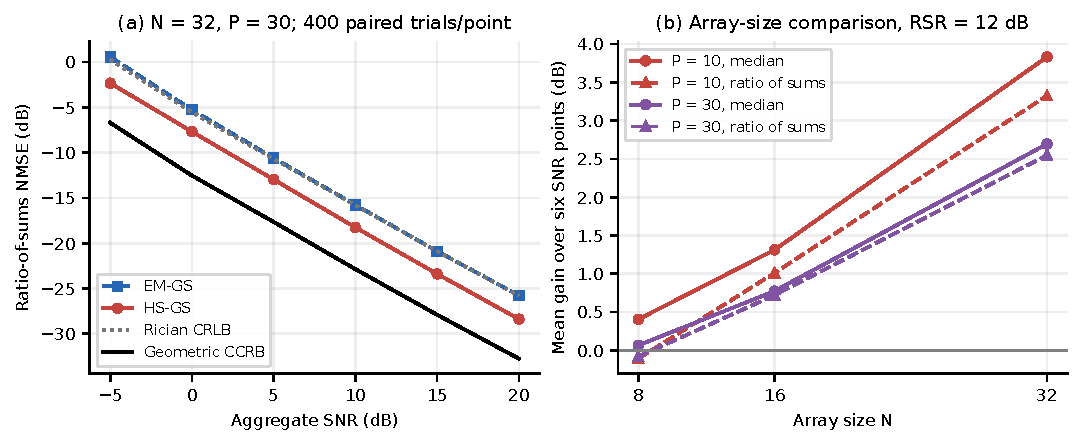
\includegraphics[width=\textwidth]{fig/figure2_performance_array.pdf}
\caption{Verified performance. (a) NMSE versus aggregate SNR for
$N=32$, $P=30$, and RSR $=12$~dB; shaded bands are pointwise 95\%
paired-bootstrap intervals. (b) HS-GS gain versus array size for two pilot
counts. Error bars are pointwise 95\% intervals.}
\label{fig:main}
\end{figure*}

\begin{table}[!t]
\caption{Array-size summary, averaged over 12 operating points (dB).}
\label{tab:array}
\centering
\footnotesize
\begin{tabular}{rrrr}
\toprule
$N$ & Ratio-of-sums gain & Paired median & EM-GS NMSE\\
\midrule
8  & $-0.095$ & $0.236$ & $-8.666$\\
16 & $0.866$  & $1.044$ & $-8.786$\\
32 & $2.938$  & $3.264$ & $-8.733$\\
\bottomrule
\end{tabular}
\end{table}

\subsection{Effect of Channel Complexity}
\label{sec:pathcount}

Fig.~\ref{fig:path} varies the common path count at $N=32$, $P=30$,
SNR $=5$~dB, and RSR $=12$~dB. The ratio-of-sums gain decreases from
7.377~dB, with a 95\% interval of $[7.162,7.607]$~dB, at $L=2$ to
$-0.125$~dB, with interval $[-0.204,-0.046]$~dB, at $L=16$. The EM-GS
baseline spans only 0.129~dB, so the trend is caused mainly by the changing
value of the structural constraint. At $L=16$, the paired median is exactly
zero because many trials fall back to EM-GS, even though aggregate squared
error is slightly worse.

\begin{figure}[!t]
\centering
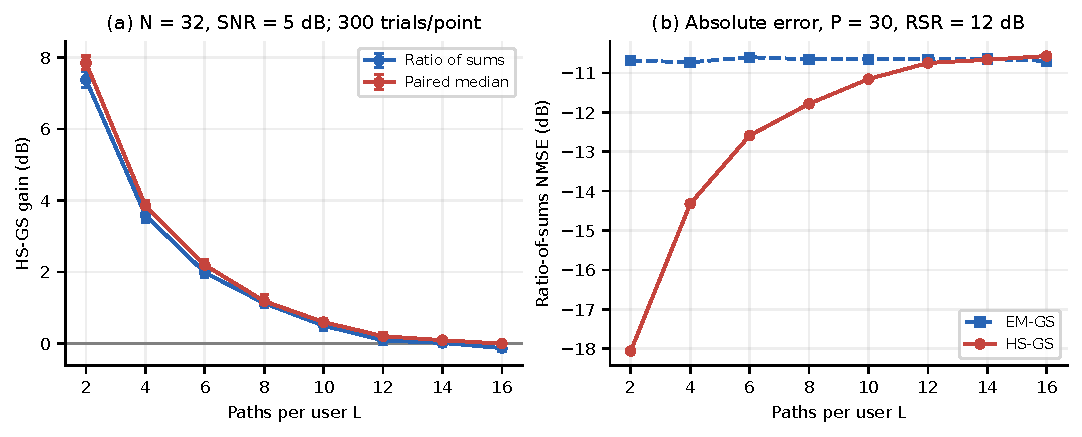
\includegraphics[width=\columnwidth]{fig/path_count.pdf}
\caption{Verified gain versus the common number of paths per user. Bars show
pointwise 95\% paired-bootstrap intervals. Structural gains are large for
sparse channels and vanish near the Hankel rank cap.}
\label{fig:path}
\end{figure}

This behavior follows from the capacity
$r_{\max}=\lceil N/2\rceil$. For $N=32$, a two-path channel occupies only a
small part of the available Hankel rank. At $L=16$, rank reduction has
little justified structure to exploit and can remove real channel
components. The result supports a mechanism-level claim within the
geometric ULA model, rather than a claim that path count alone determines
performance.

\subsection{Effective Rank and Competing Descriptors}
\label{sec:effrank}

For Hankel singular values $\{\sigma_i\}$, define
\begin{equation}
r_{\mathrm{eff}}=\exp\!\left(-\sum_i p_i\ln p_i\right),
\quad
p_i=\frac{\sigma_i}{\sum_j\sigma_j},
\quad
\rho=\frac{r_{\mathrm{eff}}}{r_{\max}}.
\end{equation}
We calculate $\rho$ from the true noiseless channel only for retrospective
analysis; the receiver does not know it before estimation.

The original unmatched experiment gives nominal zero-crossing estimates
0.580, 0.509, and 0.526 for $N=16,32,64$. The first and third are
extrapolations from positive-gain points, while only the $N=32$ value
interpolates between positive and negative ratio-of-sums estimates. They
therefore do not establish a common measured threshold.

Fig.~\ref{fig:rank} instead matches pilot count, RSR, iteration budgets,
SNR distribution, and the pooled-median statistic across array sizes.
Gain generally declines as $\rho$ rises, but the $N=32$ curve still has a
positive 0.141~dB median gain at $\rho=0.536$, with interval
$[0.090,0.211]$~dB. These data do not support a universal cutoff at
$\rho=0.5$.

\begin{figure*}[!t]
\centering
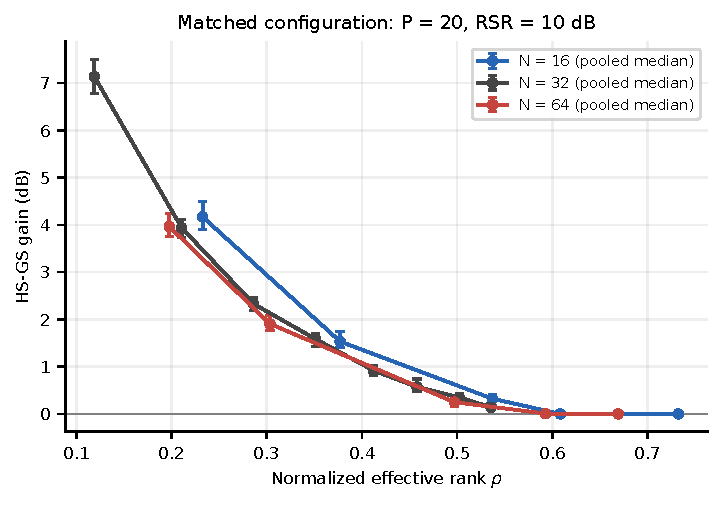
\includegraphics[width=\textwidth]{fig/figure3_matched.pdf}
\caption{Matched effective-rank experiment using $P=20$, RSR
$=10$~dB, 100/25 final/candidate updates, random aggregate SNR in
$[-10,20]$~dB, and pooled paired medians. The decline is descriptive; no
universal zero-gain threshold is established.}
\label{fig:rank}
\end{figure*}

Using the matched $N=32$ curve to predict six held-out $N=16$ and $N=64$
configurations gives mean absolute errors of 2.067~dB for raw path count,
0.073~dB for normalized path count $L/r_{\max}$, and 0.317~dB for $\rho$.
Thus $\rho$ improves on raw path count in this test, but normalized path
count is the stronger of the tested predictors. This comparison is limited
to a small geometric-channel grid and a specified piecewise-linear
interpolation; all six target gains are positive.

At $N=16$, $L=14$, and measured $\rho=0.732$, forcing rank seven gives a
median gain of $-0.154$~dB with interval $[-0.201,-0.111]$~dB. Adaptive
HS-GS has zero pooled median gain and falls back in 35.75\% of these trials.
This demonstrates the risk of forced rank reduction without implying that
held-out selection is harmless on every realization.

\subsection{Alternative Channel Distributions}

Two additional distributions retain the geometric ULA model but change
path generation. Initial complex path gains have variance $1/D$ for $D$
rays; each channel matrix is then scaled to match the realized total power
of a base draw. The clustered case uses four clusters, ten rays per cluster,
uniform $\pm5^\circ$ angular offsets, and angle clipping. The other case
uses ten independent paths.

In 400 fresh trials per distribution, the clustered channel has
$\rho=0.335$ and a 1.182~dB median gain with interval
$[0.995,1.398]$~dB. Its error relative to the previously frozen
1.300~dB prediction is 0.118~dB. The ten-path channel has $\rho=0.407$
and a 0.831~dB gain with interval $[0.710,1.011]$~dB; its error relative
to the frozen 0.648~dB prediction is 0.183~dB. These results support
positive transfer within two changed multipath distributions, but do not
establish exact calibration or transfer beyond the ULA model.

\begin{figure}[!t]
\centering
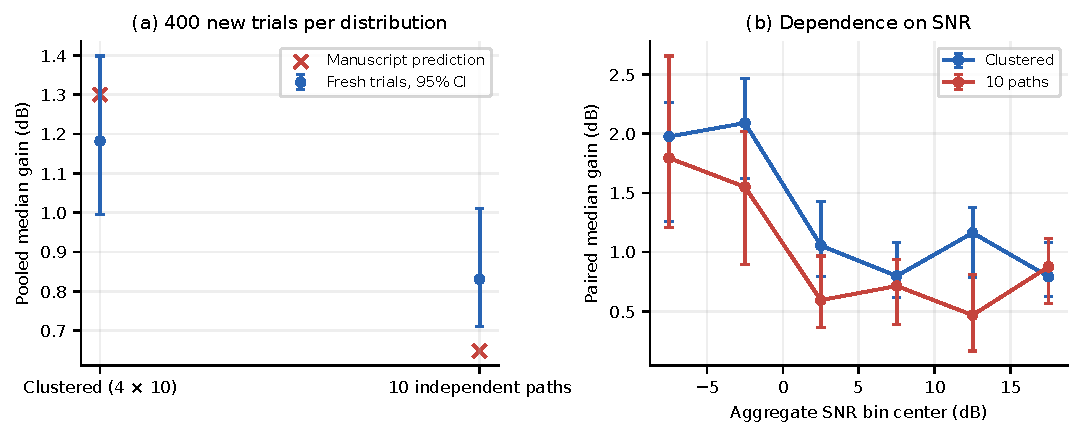
\includegraphics[width=\columnwidth]{fig/distribution_transfer.pdf}
\caption{Frozen predictions and verified gains for two alternative path
distributions. Both remain within the geometric ULA model.}
\label{fig:transfer}
\end{figure}

\subsection{Projection Placement and Computation}
\label{sec:placement}

To isolate projection placement, we compare interleaved and final-only
variants on the same 300 trials per SNR. Positive values in
Fig.~\ref{fig:placement} favor interleaving. The original comparison uses
four Cadzow sweeps after each interleaved update but one sweep at the end;
its mean of six per-SNR medians is $-0.012$~dB with interval
$[-0.049,0.034]$~dB. Because both placement and sweep count change, this
near-zero result does not establish equivalence.

With four sweeps per application in both variants, the interleaving
advantage is 0.204~dB with interval $[0.169,0.242]$~dB. With one sweep
per application in both variants, it is 0.239~dB with interval
$[0.204,0.282]$~dB. All variants share the rank selected using four-sweep
interleaved candidates, so this is a conditional comparison rather than a
separately tuned contest. Equal sweeps per application also do not equalize
total computation, because interleaving repeats the application after every
EM-GS update.

\begin{figure*}[!t]
\centering
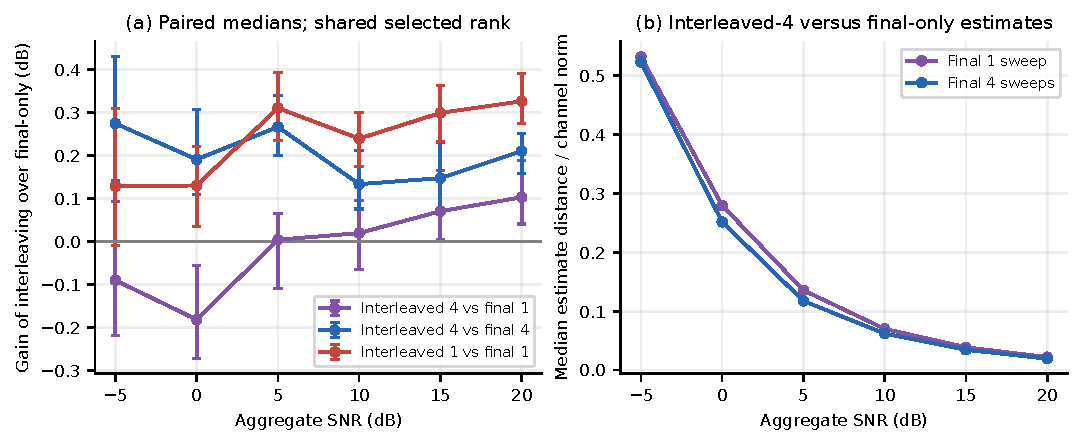
\includegraphics[width=\textwidth]{fig/projection_placement.pdf}
\caption{Controlled projection-placement study. Matching the Cadzow sweeps
per application reveals a modest interleaving advantage. The bottom panel
also shows that interleaved and final-only processing produce different
channel estimates, especially at low SNR.}
\label{fig:placement}
\end{figure*}

The median separation between the interleaved-four and final-one estimates
is 0.532 times the true-channel norm at $-5$~dB and 0.022 at 20~dB.
Consequently, applying the structural step once at the end is not
mathematically or empirically identical to interleaving it.

Serial timing on an Apple M2 with eight physical cores and 8~GiB RAM used
single-thread settings, $P=20$, SNR $=5$~dB, RSR $=10$~dB, 100 final
updates, 25 candidate updates, four sweeps, and three independent trials per
point. Median interleaved end-to-end times are 0.394, 1.059, 3.548, and
14.159~s for $N=8,16,32,64$; corresponding final-only times are
0.279, 0.874, 3.174, and 13.265~s. Rank selection accounts for 47.5\%,
65.3\%, 79.3\%, and 88.5\% of the interleaved total. These numbers describe
one implementation and machine; they are not portable complexity constants.

For completeness, at SNRs of 5~dB and above, median gains are 3.381,
3.509, and 3.552~dB for $K=2,3,4$. The associated pilot counts are
$P=13,20,27$, respectively, with $L=5$ and approximately fixed $P/(2K)$.
The 0.170~dB span therefore describes this joint design and does not isolate
user count alone.

\section{Limitations and Conclusion}

The independent simulations support using Hankel structure when a geometric
multipath channel is simple relative to the array's Hankel capacity. At the
principal operating point, HS-GS gives a 2.70~dB mean of six per-SNR paired
median gains over EM-GS. Gains increase with array size and decline with path
complexity, while forced rank reduction can be harmful near the rank cap.

Normalized effective rank is a useful retrospective coordinate, but the data
do not establish a universal cutoff. In the matched cross-array comparison,
normalized path count predicts the held-out gains more accurately than
normalized effective rank. The two alternative path distributions retain
positive gains, but both still obey the same geometric ULA model.

The controlled placement experiment answers a practical implementation
question: a single projection after EM-GS does not generally reproduce the
interleaved estimator. With matching Cadzow sweeps per application,
interleaving improves the mean per-SNR paired median by 0.20--0.24~dB in
the tested design. That modest accuracy gain comes with repeated projection
cost, although rank selection is the dominant measured cost for larger
arrays.

All results are simulation based. The study does not include measured Rydberg
hardware data, array calibration error, mutual coupling, wideband channels,
or departures from the geometric ULA observation model. Rank selection uses
one shared scalar across users, and its deterministic held-out split has not
been compared with cross-validation or information criteria. The CRLB and
CCRB are unbiased-estimator references, whereas the tested estimators may be
biased. Hardware validation and comparison with the closest learned
phase-retrieval baselines are therefore the main steps needed to establish
broader practical value.

\begin{thebibliography}{99}

\bibitem{cui2025}
M.~Cui, Q.~Zeng, and K.~Huang,
``Towards atomic MIMO receivers,''
\emph{IEEE J. Sel. Areas Commun.},
vol.~43, no.~3, pp.~659--673, 2025.

\bibitem{gong2025mag}
T.~Gong \emph{et al.},
``Rydberg atomic quantum receivers for classical wireless communication and sensing,''
\emph{IEEE Wireless Commun.},
vol.~32, no.~5, pp.~90--100, 2025.

\bibitem{gerchberg1972}
R.~W.~Gerchberg and W.~O.~Saxton,
``A practical algorithm for the determination of phase from image and diffraction plane pictures,''
\emph{Optik},
vol.~35, pp.~237--246, 1972.

\bibitem{xiao2026}
J.~Xiao, J.~Wang, M.~Zeng, H.~Xu, X.~Li, and A.~Nallanathan,
``Channel estimation for Rydberg atomic quantum receivers:
unrolled phase retrieval from holographic snapshots,''
\emph{IEEE Signal Process. Lett.},
vol.~33, pp.~1696--1700, 2026.

\bibitem{xu2025}
B.~Xu, J.~Zhang, Z.~Chen, B.~Cheng, Z.~Liu, Y.-C.~Wu, and B.~Ai,
``Channel estimation for Rydberg atomic receivers,''
\emph{IEEE Wireless Commun. Lett.},
vol.~14, no.~9, pp.~2957--2961, 2025.

\bibitem{balan2015}
R.~Balan,
``The Fisher information matrix and the Cram\'er--Rao bound in a non-AWGN model for the phase retrieval problem,''
in \emph{Proc. Int. Conf. Sampling Theory Appl. (SampTA)},
2015.

\bibitem{chen2014emac}
Y.~Chen and Y.~Chi,
``Robust spectral compressed sensing via structured matrix completion,''
\emph{IEEE Trans. Inf. Theory},
vol.~60, no.~10, pp.~6576--6601, 2014.

\bibitem{jin2016aloha}
K.~H.~Jin, D.~Lee, and J.~C.~Ye,
``A general framework for compressed sensing and parallel MRI using annihilating filter based low-rank Hankel matrix,''
\emph{IEEE Trans. Comput. Imag.},
vol.~2, no.~4, pp.~480--495, 2016.

\bibitem{haldar2014loraks}
J.~P.~Haldar,
``Low-rank modeling of local $k$-space neighborhoods (LORAKS) for constrained MRI,''
\emph{IEEE Trans. Med. Imag.},
vol.~33, no.~3, pp.~668--681, 2014.

\bibitem{tang2013offgrid}
G.~Tang, B.~N.~Bhaskar, P.~Shah, and B.~Recht,
``Compressed sensing off the grid,''
\emph{IEEE Trans. Inf. Theory},
vol.~59, no.~11, pp.~7465--7490, 2013.

\bibitem{cadzow1988}
J.~A.~Cadzow,
``Signal enhancement---a composite property mapping algorithm,''
\emph{IEEE Trans. Acoust., Speech, Signal Process.},
vol.~36, no.~1, pp.~49--62, 1988.

\bibitem{markovsky2008}
I.~Markovsky,
``Structured low-rank approximation and its applications,''
\emph{Automatica},
vol.~44, no.~4, pp.~891--909, 2008.

\bibitem{royvetterli2007}
O.~Roy and M.~Vetterli,
``The effective rank: a measure of effective dimensionality,''
in \emph{Proc. Eur. Signal Process. Conf. (EUSIPCO)},
2007, pp.~606--610.

\bibitem{gorman1990}
J.~D.~Gorman and A.~O.~Hero,
``Lower bounds for parametric estimation with constraints,''
\emph{IEEE Trans. Inf. Theory},
vol.~36, no.~6, pp.~1285--1301, 1990.

\bibitem{stoica1998}
P.~Stoica and B.~C.~Ng,
``On the Cram\'er--Rao bound under parametric constraints,''
\emph{IEEE Signal Process. Lett.},
vol.~5, no.~7, pp.~177--179, 1998.

\end{thebibliography}

\end{document}
